\section{Materials}
\subsection{Plastic for lasercutting}
For this project we got a bunch of different plastic materials from RIAS, in order to find some material that might be cheaper, and better that acrylic, since acrylic have tendency to be brittle, this becomes worse when it has been laser cut\cite{AcrylTension}.
all of the plastic was thermoplastic, which is a term for a specific type of plastic\ref{Thermoplastic} that is used in the laser industry.
For the laser cutter we made some simple figures to see what the result would be.
The requirements for the material is that it is easy to lasercut, and don't break easy.

\subsubsection{PEHD}
The first material that we tried to cut was, PEHD (as shown in figure \ref{fig:PEHD}) which is used in the production of ex. plastic bottles and corrosion-resistant piping it is known for having a high strength to density ratio.
The cutting went fine, but there was some residue left over from the cutting, that we had some problems removing.
% There ware some problems getting the resedu off the plastic after the cutting, also the material have a tendensy to hold it's form when bent.%

\begin{figure}[h]
\begin{minipage}[b]{7.5cm}
\centering
	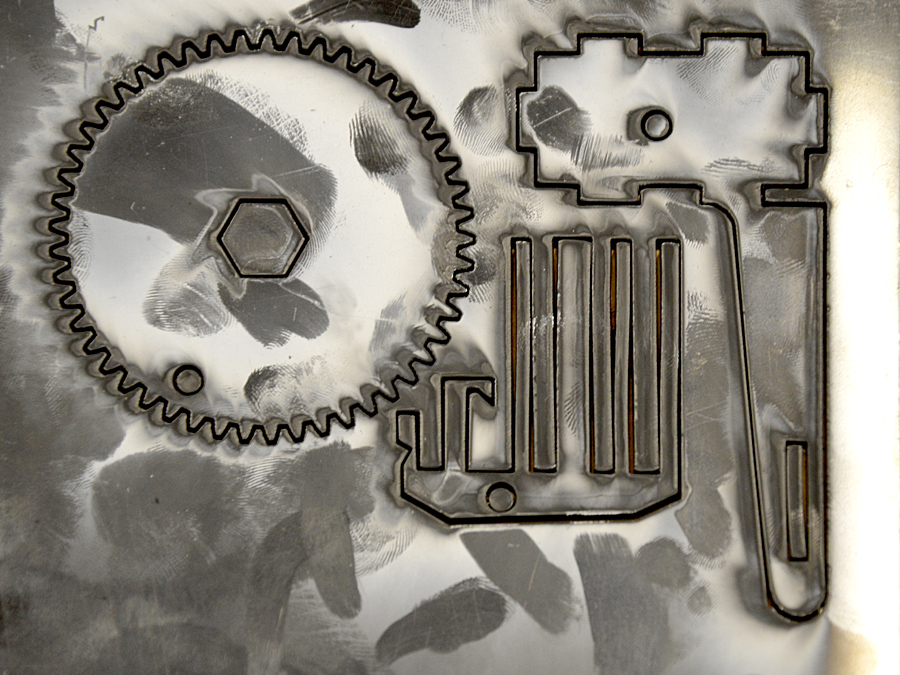
\includegraphics[scale=1.0]{figures/PEHD.jpg}
	\caption{\small {\it {Cut test of PEHD}}} \label{fig:PEHD}
\end{minipage}
\begin{minipage}[b]{7.5cm}
\centering
	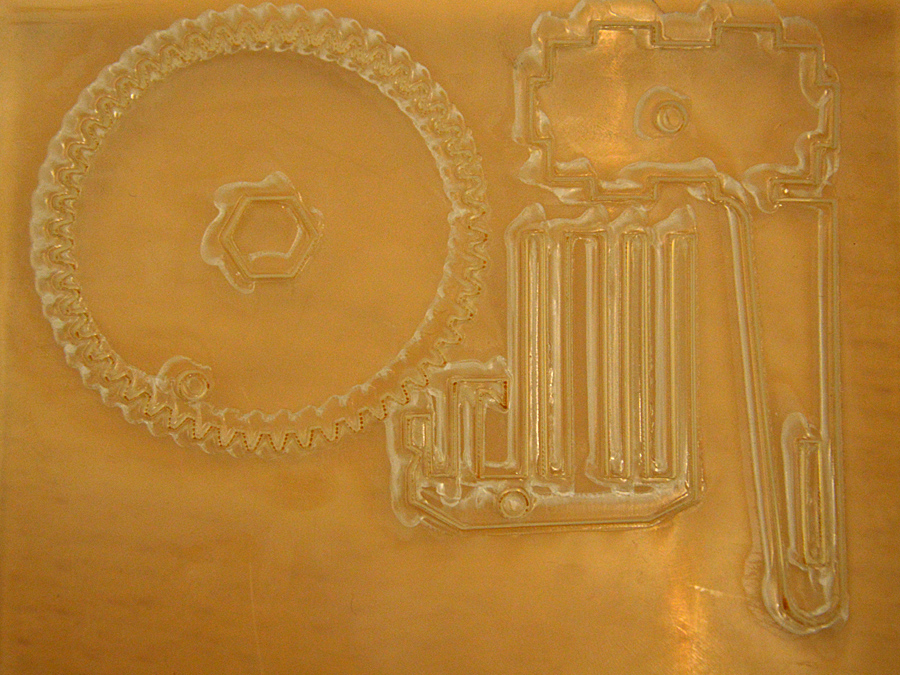
\includegraphics[scale=1.0]{figures/PP.jpg}
	\caption{\small {\it {Cut of RIALEN PP}}} \label{fig:PP}
\end{minipage}
\end{figure}

% \begin{figure}[!h]
% 	\centering
% 	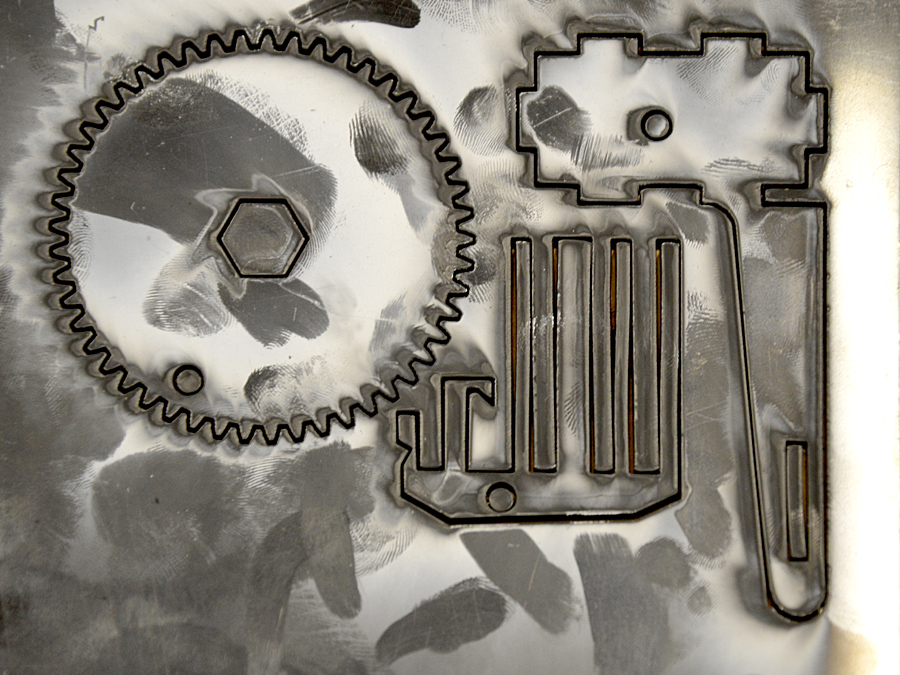
\includegraphics[scale=1.0]{figures/PEHD.jpg}
% 	\caption{\small {\it {Cut test of PEHD}}} \label{fig:PEHD}
% \end{figure}
% \FloatBarrier

\subsubsection{PP}
 PP (as shown in figure \ref{fig:PP}) is most commonly used in packaging and labeling, and it has resistant to many chemical solvents, bases and acids.
The cutting had some big problems, one of them was that after 3 cutting rounds, the laser still haven't cut through the material, which meant we had to let it be, and not trying to cut in that material.

% \begin{figure}[!h]
% 	\centering
% 	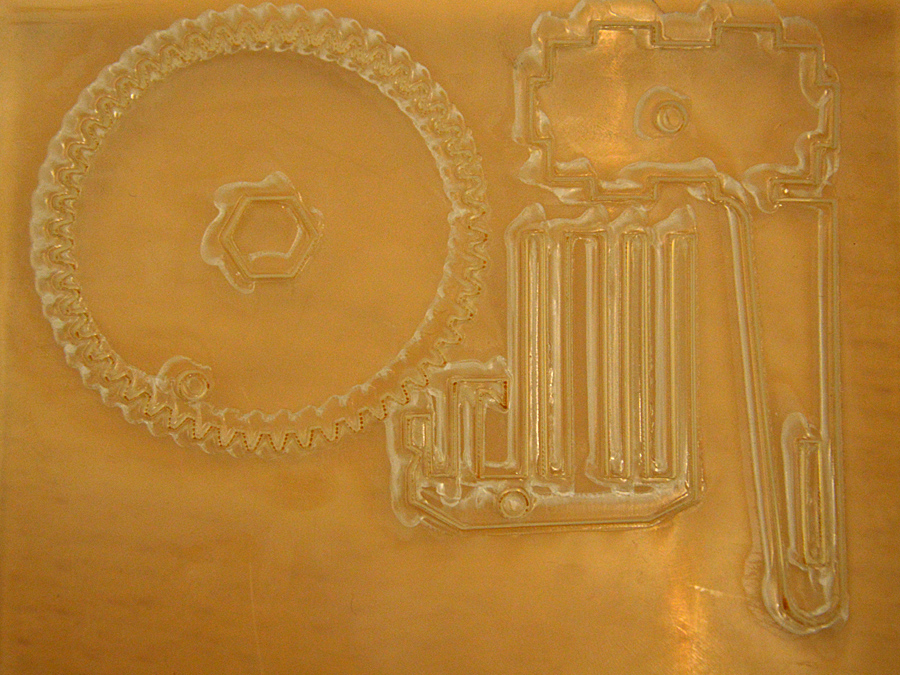
\includegraphics[scale=1.0]{figures/PP.jpg}
% 	\caption{\small {\it {Cut of RIALEN PP}}} \label{fig:PP}
% \end{figure}
% \FloatBarrier

\subsubsection{PP-H}
Is PP (as shown in figure \ref{fig:PP-H}) where they have added Homopolymer to, this changes the materials propertyes, so it is becomes easier to cut, but it leaves some residue when cut, it also have tendency to curl up on it self, where it has been cut.
However the material has memory, which means that it remember the shape is has been bend, this is a problem since we are going to have some eletronic attach to it.

\begin{figure}[h]
\begin{minipage}[b]{7.5cm}
	\centering
	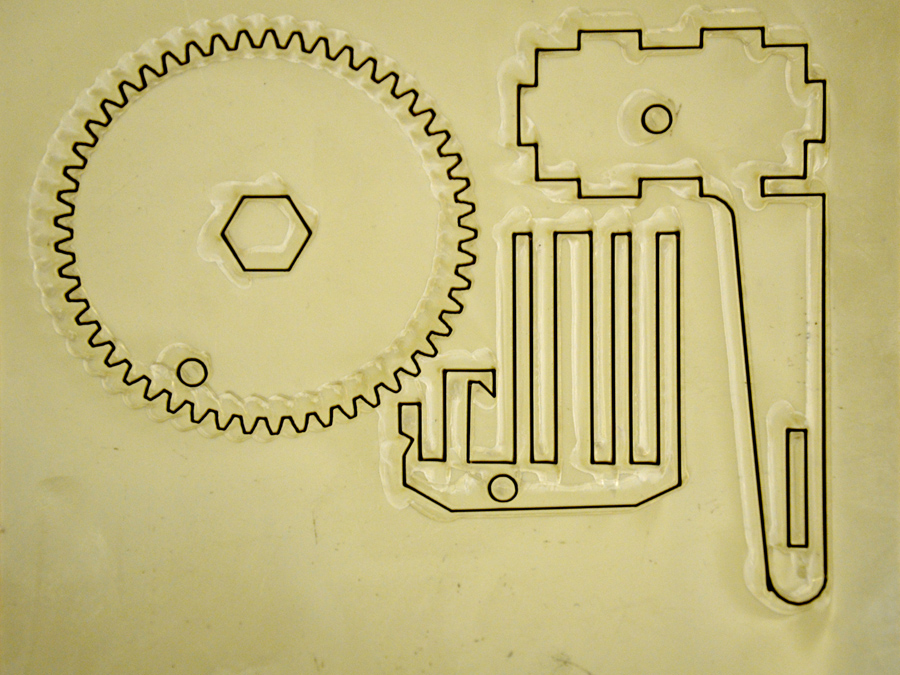
\includegraphics[scale=1.0]{figures/PP-H.jpg}
	\caption{\small {\it {Cut test of PP-H}}} \label{fig:PP-H}
\end{minipage}
\begin{minipage}[b]{7.5cm}
	\centering
	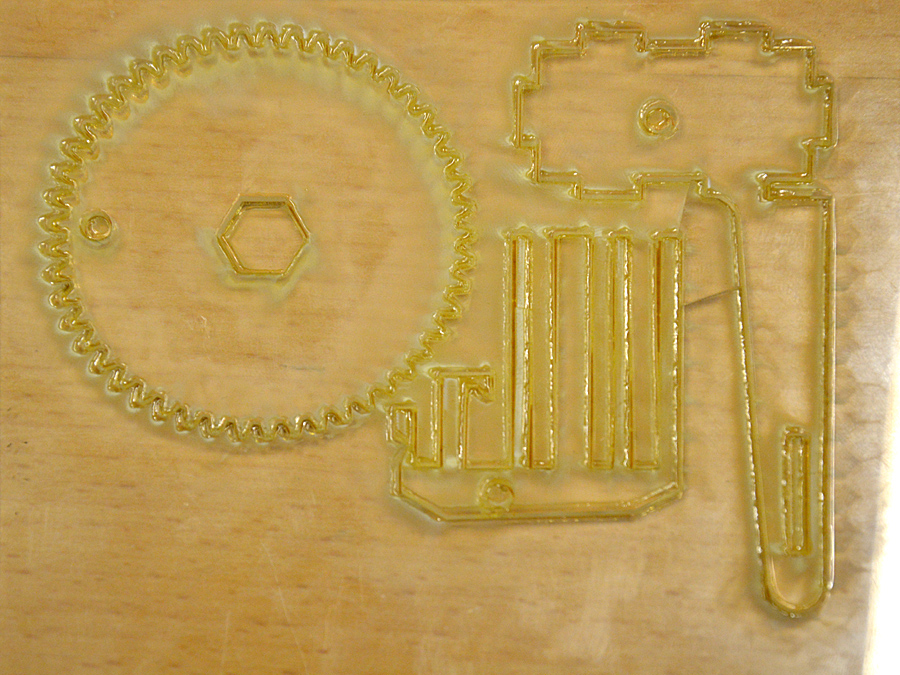
\includegraphics[scale=1.0]{figures/PETG.jpg}
	\caption{\small {\it {Cut test of PETG}}} \label{fig:PETG}
\end{minipage}
\end{figure}

\begin{figure}[!h]
	\centering
	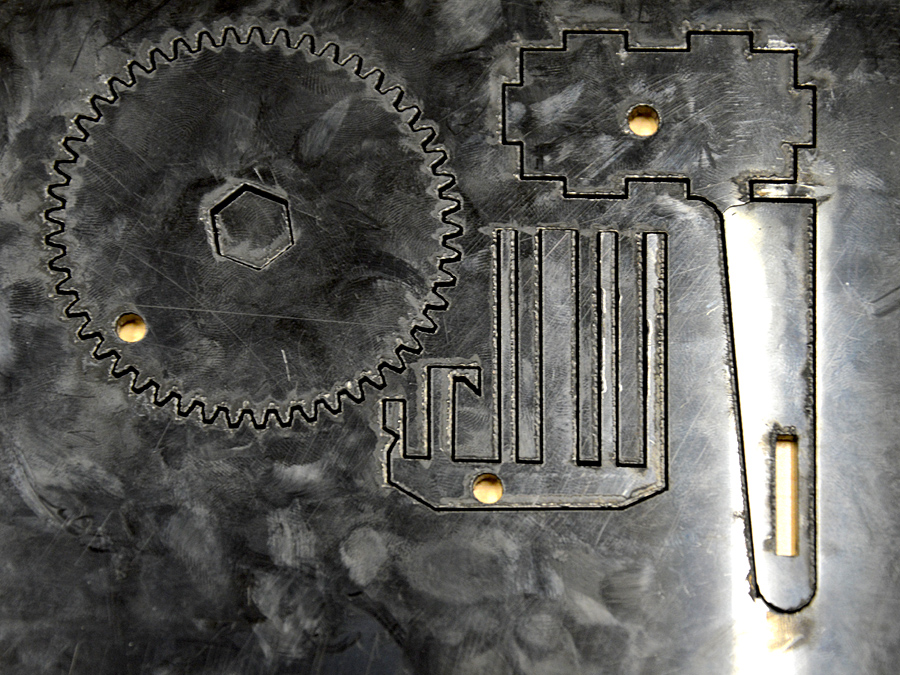
\includegraphics[scale=1.0]{figures/POM-C.jpg}
	\caption{\small {\it {Cut test of POM-C}}} \label{fig:POM-C}
\end{figure}
\FloatBarrier

\subsubsection{PETG}
PETG (as shown in figure \ref{fig:PETG}) is used alot in the production of plastic bottles, and is a durable material.
The cutting process did not go as hoped, be side that one can see the burn marks, it also had a very strong chemical smell, that took weeks to dissipate.

\subsubsection{POM-C} 
POM-C (as shown in figure \ref{fig:POM-C})  is a material that works well with laser cutting, it is used commonly in small gear wheels, ball bearings, and many other product where you need low friction and stiffness.
The cutting of it went fine, but we found out that if we want to use it, we may have some problems since the glue, that is used for it is highly toxic, furthermore the material more expensive compared to Acrylic.

\subsubsection{PEEK}
PEEK is one of the materials that we would have liked to try out since it is one of the materials that are used in the medical industry, however it is an expensive material and it is hard to get in sheets, we did have some conversion over mail with RIAS, but was unable to secure some samples.

\subsubsection{ACRYL}
Acrylic is a easy material to use in a laser cutter, the biggest problem with it, is that it is brettle, and does have a tendency to break when it hits something hard or comes under tension.
we did not try to make test cuts in it, since we have cut a lot of acrylic and know the properties of it.


\subsubsection{Conslusion}
The conclusion is that we are going to use acrylic, since we have easy accesse to it and it's cheap, and can try to mend the disadvantages.

\subsection{Plastic for 3D printing}
There are 2 commenly used plastic for 3D printing PLA and ABS \cite{PLAABS}

\subsubsection{PLA}
PLA (poly lactic acid) is a bio-degradable plastic that is mostly made from corn starch or sugar cane.
It has a lower melting point that ABS, and can be printed on a cold surcafe. you can also print faster with highere presision. you don't need a ventelated room like abs, since it does not produce plastic fumes. And it is food safe.

However it is less sturdy, have a shorter lifespan that ABS. Since it has a lower melting point that ABS it can deform when heated Ex. hot water will deform it.

\subsubsection{ABS}
ABS (Acrylonitrile Butadiene Styrene) is made from oil, and has a highere melting temperture than pla, it also have highere strength and flexibility and a logerlifespan, which is the reason that it is used in Ex. LEGO

It does have some downside, it deformes when you don't print in on an hot surface, which makes it harder to print. It gives out plastic fumes when printed, so you need a ventilated room, and it is not suitable if you going to use it with food.

\subsubsection{Conslusion}
We have chosen to use PLA, since the rooms where the printers are, arn't ventilated.

